\chapter{Basics}

\section{Historical background}
(Tự đọc)

\section{Components and Terms}

\subsection{Purpose of Computer Networks}

\noindent
General task: enable communication among paticipants.

\begin{itemize}
    \item Resource sharing: assign different tasks to different computers $\rightarrow$ Chia sẻ tài nguyên để tránh bị nghẽn.
    \item Resource pooling: make multiple small computers act like one large powerful system $\rightarrow$ Gộp tài nguyên thành một cụm để chạy tốt hơn.
    \item Resource balancing: increase the availability of the service by redundancy $\rightarrow$ thay vì 1 máy chạy thì nó sẽ duplicate ra cho nhiều máy $\Rightarrow$ khi có lỗi thì còn mấy thằng khác để chạy.
\end{itemize}
\medskip

\subsection{Requirement Components to set up a Computer Network}

\noindent
Phải có 3 yếu tố chính:

\begin{enumerate}
    \item Computers $\rightarrow$ phải có $\geq$ 2 máy tính trở lên.
    \item Transmission medium $\rightarrow$ phải có cho nhận (send/receive); có 2 hình thức: \textbf{có dây} (wire) và \textbf{không dây} (wireless).
    \item Network protocols $\rightarrow$ phải có cách giao thức, như là luật để tụi nó giao tiếp với nhau.
\end{enumerate}

\medskip

\subsection{Network Services}

\noindent
Network service $\rightarrow$ cung cấp tài nguyên cho các thiết bị khác trong cái network đó.
\medskip

\noindent
Distinguished by their role:
\begin{itemize}
    \item Server (máy chủ) $\rightarrow$ hold secures (file, database, etc.) and wait for requests from others $\Rightarrow$ provide a network service.
    \item Client (máy khách) $\rightarrow$ send a request to the server and waits for the response $\Rightarrow$ uses (consumes) a network service.
\end{itemize}
\medskip

\noindent
Peer-to-peer networks (mạng ngang hàng) $\rightarrow$ every computer can download files from others (client role) and upload files to other (server role) at the same time.
\medskip

$\Rightarrow$ Nói nôm na là, mạng peer-to-peer là là tụi nó cứ liên tục swap role cho nhau, tụi nó ở ngang hàng nhau, không thằng nào hơn role thằng nào cả.
\medskip

\vspace{0.2cm}

\noindent
$\Rightarrow$ Chú ý: các thuật ngữ như "server", "client", "peer" chỉ dùng cho network và không đụng đến phần cứng.

\subsection{Transmission Media}

\noindent
Có 2 loại truyền:

\begin{itemize}
    \item Guided transmission media (là truyền bằng dây).
    \item Wireless transmission.
\end{itemize}

\noindent
Wireless transmission có 2 cách là \textbf{directed} và \textbf{undirected}:

\begin{itemize}
    \item Directed (có hướng) $\rightarrow$ must aim hardware physically.
    \item Undirected (đa hướng) $\rightarrow$ no aiming needed.
\end{itemize}

\noindent
\textbf{Bonus:} In security problem:

\begin{itemize}
    \item Directed $\rightarrow$ harder to intercept.
    \item Undirected $\rightarrow$ easier to intercept.
\end{itemize}
\medskip

\noindent
Directed transmission technologies:

\begin{itemize}
    \item Radio technology.
    \item Infrared.
    \item Laser.
\end{itemize}

\noindent
Undirected wireless transmission $\rightarrow$ mostly based on radio technology (WLAN, cellular networks, etc.).
\medskip

\subsection{Protocols}

\noindent
Protocol $\rightarrow$ set of all previously made agreements between communication partners:

\begin{itemize}
    \item Connection establishment \& termination.
    \item Synchronization.
    \item Error detection.
    \item Vocabulary $\rightarrow$ valid messages.
    \item Encoding.
\end{itemize}

\noindent
$\Rightarrow$ Specifies the syntax (message valid format) and semantics (vocabulary and meaning of valid messages).
\medskip

\noindent
\underline{Self-note:} Tại sao lại phải cần check coi có đúng "semantic" (nghĩa là xem coi nó nghe có hợp lý) không? 

$\rightarrow$ Thử tưởng tượng ha, câu "tôi ăn đá" vẫn đúng cấu trúc ngữ pháp, tuy nhiên là trên thực tế câu này nghe rất vô lý $\Rightarrow$ chính vì thế nên mới phải check semantics.
\medskip

\subsection{Computer Networks Distinguished by their Dimension}

\noindent
\underline{Self-note:}

\begin{itemize}
    \item PAN (Personal Area Network) $\rightarrow$ for personal use within a user's intermediate workspace.
    \item BAN (Body Area Network) $\rightarrow$ specifically centered around the human body.
\end{itemize}

\noindent
$\Rightarrow$ Nói tóm lại: đây là network có vùng phủ nhỏ (few meters), thường có trong các điện thoại thông minh.
\medskip

\subsubsection{Local Area Network (LAN)}

\begin{itemize}
    \item Local network.
    \item Range: appartment, building, company site, or university campus.
    \item Dimension: 500-1000 m.
\end{itemize}

\subsubsection{Metropolitan Area Network (MAN)}

\begin{itemize}
    \item Connects LANs.
    \item Range: a city, or agglomeration area (khu có nhiều dân cư).
    \item Dimension: 100 km.
\end{itemize}

\subsubsection{Wide Area Network (WAN)}

\begin{itemize}
    \item Connects serveral networks.
    \item Range: large geographic inside a country or continent.
    \item Dimension: 1000 km.
\end{itemize}

\noindent
So sánh về độ phủ sóng: LAN < MAN < WAN.
\medskip

\subsection{Unicast and Broadcast}

\subsubsection{Unicast}

\noindent
One-to-one communication.

\begin{figure}[h]
    \centering
    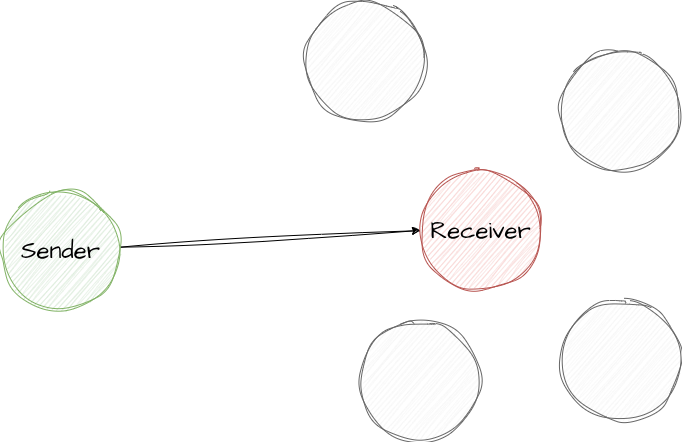
\includegraphics[width=0.5\textwidth]{assets/chap_1/unicast.png}
\end{figure}

\subsubsection{Broadcast}

\noindent
One-to-all communication.

\begin{figure}[h]
    \centering
    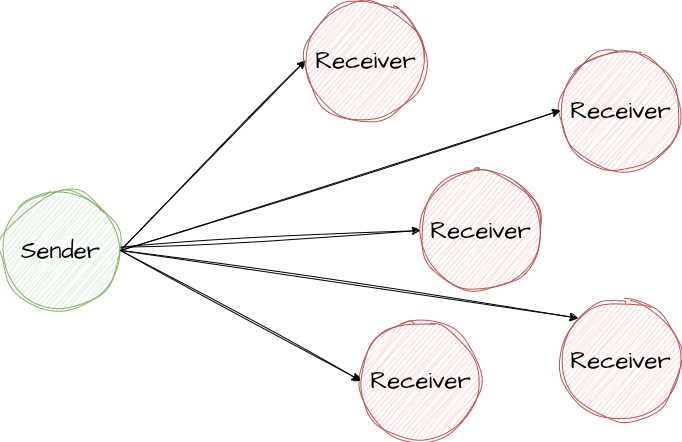
\includegraphics[width=0.5\textwidth]{assets/chap_1/broadcast.png}
\end{figure}

\subsection{Group Communication: Multicast and Anycast}

\noindent
\underline{Self-note:} Multicast và anycast ở đây chỉ gửi cho nhóm, nhưng multicast thì gửi mọi người trong nhóm, còn anycast thì chỉ gửi cho một người bất kỳ trong nhóm thôi.
\medskip

\subsubsection{Multicast}

\noindent
One-to-group communication (group communication).

\begin{figure}[h]
    \centering
    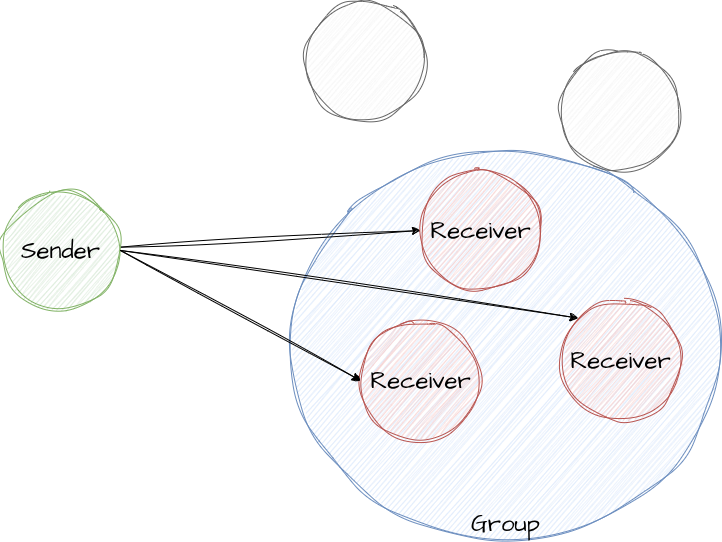
\includegraphics[width=0.5\textwidth]{assets/chap_1/multicast.png}
\end{figure}

\subsubsection{Anycast}

\noindent
One-to-any communication.

\begin{figure}[h]
    \centering
    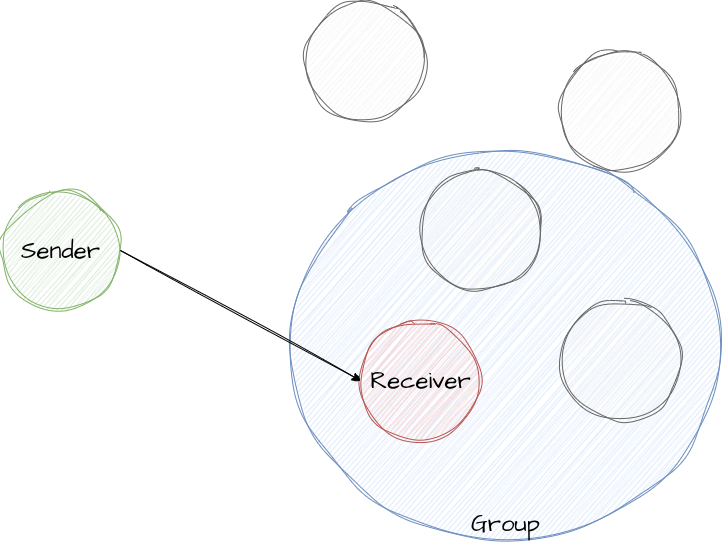
\includegraphics[width=0.5\textwidth]{assets/chap_1/anycast.png}
\end{figure}
\medskip

\noindent
\underline{Self-note:} Unicast và broadcast gửi cho từng người một, khác với multicast và anycast là gửi cho nhóm $\rightarrow$ khác nhau giữa gửi không trong nhóm và gửi trong nhóm.
\medskip

\subsection{Connection-Orientation}

Có 2 phương thức: \textbf{connection-oriented} (có kết nối) và \textbf{connectionless} (phi kết nối).

\subsubsection{Connection-Oriented}

\noindent
$\rightarrow$ The service operates \textbf{stateful} (có trạng thái).
\medskip

\begin{itemize}
    \item Three phases: connection establishment, data transfer, connection termination.
    \item Virtual path between the involved hosts is established.
    \item Sequent data is exchanged between the same hosts.
\end{itemize}

\noindent
$\rightarrow$ Server, hoặc thiết bị mạng, lưu trữ thông tin về các session hoặc connection đang diễn ra $\Rightarrow$ cung cấp khả năng lọc \& quản lý connection thông minh hơn.
\medskip

\subsubsection{Connectionless}

\noindent
$\rightarrow$ The service operates \textbf{stateless} (không trạng thái).

\begin{itemize}
    \item No path between the involved hosts is established.
\end{itemize}

\noindent
$\rightarrow$ Xử lý từng yêu cầu một cách độc lập mà không cần ghi nhớ các yêu cầu trước đó $\Rightarrow$ đơn giản và nhanh hơn do không có overhead để theo dõi.
\medskip

\noindent
\underline{Self-note:} Overhead nghĩa là phần tốn thêm để được truyền đi đúng cách, là mấy cái như header, trailer của gói tin chẳng hạn.
\medskip

\subsection{Directional Dependence (Anisotropy) of Data Transmission}

\noindent
\underline{Self-note:} Anisotropy nghĩa là tính định hướng.
\medskip

\noindent
Directional có 3 chế độ truyền (communication modes): \textbf{simplex}, \textbf{half-duplex}, và \textbf{full-duplex}.
\medskip

\noindent
A communication channel with two (or more) endpoints:

\begin{itemize}
    \item Simplex (đơn công) $\rightarrow$ chỉ có một bên có thể gửi tính hiệu.
    \item Full-duplex (song công toàn phần) $\rightarrow$ cả hai bên đều có thể gửi và nhận cùng lúc (simultaneously).
    \item Half-duplex (bán song công) $\rightarrow$ mỗi bên chỉ có thể gửi và nhận nhưng không cùng thời điểm với nhau được.
\end{itemize}

\noindent
\underline{Self-note:} Endpoint có nghĩa là điểm giao tiếp.
\medskip

\subsection{Bandwidth, Throughput and Goodput}

\noindent
Các yếu tố ảnh hưởng trong network:

\begin{itemize}
    \item Bandwidth (băng thông) $\rightarrow$ throughput.
    \item Latency (độ trễ).
\end{itemize}
\medskip

\noindent
\textbf{Mở rộng định nghĩa:}

\begin{itemize}
    \item Bandwidth: băng thông $\rightarrow$ là khả năng mà đường truyền mạng có thể truyền dữ liệu trong 1 giây.
    \item Throughput: thông lượng $\rightarrow$ là tốc độ thực tế được truyền qua mạng trong một khoảng thời gian, bao gồm tổng số bit đã truyền, kể cả những bit truyền không thành công.
    \item Goodput: thông lượng hữu ích $\rightarrow$ đo lường tốc độ dữ liệu hữu ích mà một ứng dụng nhận được trên mạng, remove phần dữ liệu dư thừa (actual achieved data rate); chẳng hạn như các bit dư thừa, hoặc các gói bị mất hay truyền lại.
\end{itemize}
\medskip

\underline{Self-note:} goodput $\le$ throughput.

\subsection{Latency}

\noindent
Latency (độ trễ) $\rightarrow$ là khoảng thời gian một gói tin mất để đi từ nơi gửi (sender) đến nơi nhận (receiver).
\medskip

\noindent
\textbf{Công thức:}

\begin{equation*}
    \text{Latency} = \text{Propagation delay} + \text{Transmission delay} + \text{Waiting time}
\end{equation*}

\begin{equation*}
    \text{Propagation delay} = \frac{\text{Distance}}{\text{Speed of light} * \text{Velocity factor}}
\end{equation*}
\medskip

\noindent
Chú giải:

\begin{itemize}
    \item Distance: khoảng cách giữa sender và receiver trong cái network connection.
    \item Speed of light: tốc độ ánh sáng.
    \item Velocity factor: hệ số vận tốc $\rightarrow$ nó là hệ số cụ thể, ra thi đề sẽ cho; ví dụ: Vacuum (môi trường chân không) là 1.
\end{itemize}
\medskip

\begin{equation*}
    \text{Transmission delay} = \frac{\text{Message size}}{\text{Bandwidth}}
\end{equation*}
\medskip

\noindent
\textbf{Lưu ý:}

\begin{itemize}
    \item Nếu message chỉ có single bit $\rightarrow$ transmission delay = 0.
    \item Nó cần phải cache receive data (nhận dữ liệu về cache để lưu trữ) trước khi forward.
    \item Waiting time $\rightarrow$ bị gây ra do network devices (chẳng hạn như Switch).
    \item Nếu network connection giữa điểm gửi và điểm nhận chỉ là một đường thẳng hoặc một kênh truyền duy nhất $\rightarrow$ waiting time = 0.
\end{itemize}
\medskip

\section{Reference Models}

\noindent
\underline{Self-note:} Reference model nghĩa là mô hình tham chiếu 
\medskip

\noindent
Reference models $\rightarrow$ mô tả cách hoạt động của computer network một cách tổng quát, không phụ thuộc vào công nghệ cụ thể (như hardware hay software).
\medskip

\noindent
\textbf{Cách thức hoạt động:}

\begin{itemize}
    \item Mô tả network độc lập với công nghệ (mấy cái hardware/software) $\rightarrow$ nói lên tầng này làm những công việc gì (không quan tâm đến việc sử dụng ngôn ngữ lập trình gì, etc.) $\Rightarrow$ có thể quy được cùng mô hình tham chiếu để communicate với nhau.
    \item Decomposition (chia nhỏ vấn đề khó) $\rightarrow$ mô hình chia thành các phần nhỏ gọi là tầng (layers) $\Rightarrow$ mỗi tầng chỉ giải quyết một vấn đề duy nhất, tự xử lý dữ liệu của mình, và đóng gói (encapsulation) trước khi move đến các tầng khác.
    \item Modularity (tính linh hoạt và thay thế được) $\rightarrow$ có thể sửa đổi hoặc thay thế protocol ở một tầng mà không bị hư toàn bộ system.
    \item Interfaces \& Services (giao diện \& dịch vụ) $\rightarrow$ quy định các tầng rõ ràng để giao tiếp như tầng dưới sẽ cung cấp gì cho tầng trên sử dụng và ngược lại.
\end{itemize}
\medskip

\noindent
$\Rightarrow$ Tạo ra một tiêu chuẩn chung để có thể connect và thay đổi linh hoạt.
\medskip

\vspace{0.2cm}

\noindent
2 reference models phổ biến:

\begin{itemize}
    \item TCP/IP reference model $\rightarrow$ có 4 layers.
    \item ISO/OSI reference model $\rightarrow$ có 7 layers.
\end{itemize}
\medskip

\subsection{"Philosopher-Translator-Secretary" Architecture}

\begin{figure}[h]
    \centering
    \begin{tikzpicture}
        \node[inner sep=0] (img) {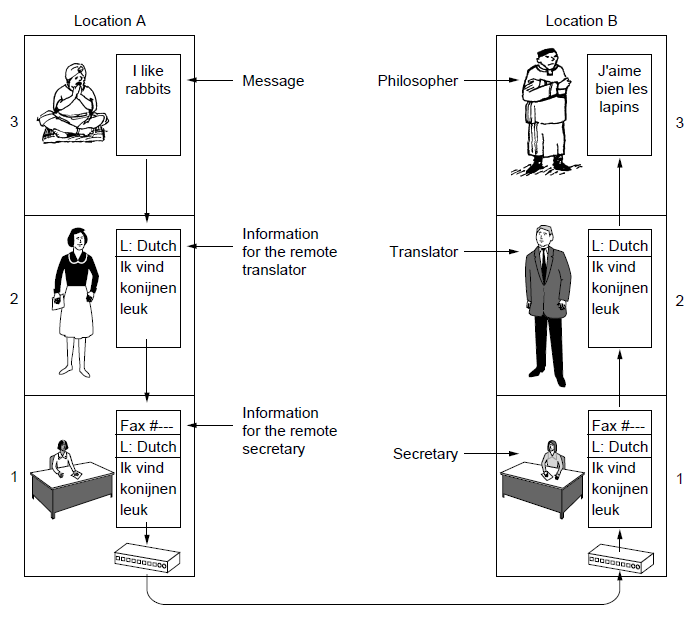
\includegraphics[width=0.5\textwidth]{assets/chap_1/philo_trans_secret.png}};
        \draw[->, ultra thick]
            ([xshift=-8mm]img.west) ++(0,1.5cm) -- ++(0,-3cm)
            node[midway, left]{Encapsulation};
        \draw[->, ultra thick]
            ([xshift=8mm]img.east) ++(0,-1.5cm) -- ++(0,3cm)
            node[midway, right]{Decapsulation};
    \end{tikzpicture}
\end{figure}

\noindent
$\rightarrow$ Ví dụ này mô tả cách giao tiếp bằng việc lấy tiếng Hà Lan làm protocol để đóng gói và đưa thông tin $\Rightarrow$ Layered Architecture.
\medskip

\subsection{TCP/IP Reference Model or DoD Model}

\noindent
\underline{Self-note:} IP nghĩa là Internet Protocol.
\medskip

\noindent
For each layer, it is specified, what functionality it provides.
\medskip

\noindent
TCP: Transmission Control Protocol $\rightarrow$ like Certified Mail: guarantees that the recipient gets the package, and send receipt back $\Rightarrow$ if lost, it will re-send.

\begin{equation*}
    \text{syn} \rightarrow \text{syn-ack} \rightarrow \text{ack received}
\end{equation*}
\medskip

\noindent
UDP: User Datagram Protocol $\rightarrow$ like sending post card: drop in mailbox and hope it arrives $\Rightarrow$ faster and cheaper, but no confirmation receipt, and may lost.
\medskip

\noindent
\textbf{Has 4 layers:}

\begin{itemize}
    \item Application Layer $\rightarrow$ contains protocols that interact directly with programs $\Rightarrow$ format the actual "payload".
    \item Transport Layer $\rightarrow$ connects applications on different devices $\Rightarrow$ chops data into manageable pieces called segments.
    \item Internet Layer $\rightarrow$ handles logical addressing and routing; pack the segments into packets.
    \item Link Layer $\rightarrow$ handles physical transmission errors and control access to the wire/air; uses physical address (MAC address).
\end{itemize}

\subsection{TCP/IP Model - Message Structure}

\begin{figure}[h]
    \centering
    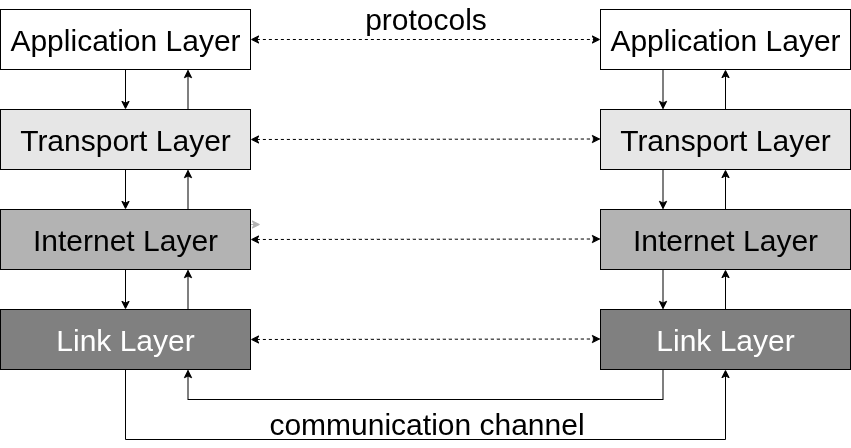
\includegraphics[width=0.5\textwidth]{assets/chap_1/TCP_IP_Struct.png}
\end{figure}
\medskip

\noindent
Each layer adds additional information as header to the message.
\medskip

\begin{itemize}
    \item Có một số protocol có link layer không chỉ có header mà còn có trailer phía cuối message; ví dụ như Ethernet.
    \item Receiver phân tích header (và trailer nếu có) trên cùng layer.
\end{itemize}
\medskip

\begin{figure}[h]
    \centering
    \begin{minipage}{0.5\textwidth}
        \centering
        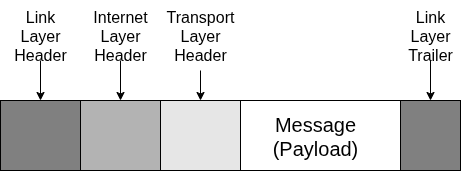
\includegraphics[width=\textwidth]{assets/chap_1/tcp_struct.png}
    \end{minipage}
    \hfill
    \begin{minipage}{0.35\textwidth}
        \centering
        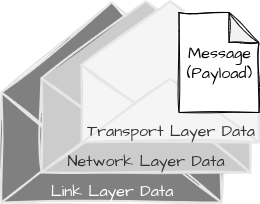
\includegraphics[width=\textwidth]{assets/chap_1/visual_email.png}
    \end{minipage}
\end{figure}
\medskip

\begin{itemize}
    \item Link Layer Header (or Link Layer) $\rightarrow$ check MAC (physical address).
    \item Internet Layer Header $\rightarrow$ check IP address.
    \item Transport Layer Header $\rightarrow$ check port number.
    \item Application Layer Header (Message/Payload) $\rightarrow$ content layer.
    \item Link Layer Trailer (nếu có) $\rightarrow$ checksum (or frame check sequence) $\Rightarrow$ error checking.
\end{itemize}

\noindent
\underline{Self-note:}

\begin{itemize}
    \item Trong cái Link Layer Header, cái header đó để check gói tin đang gọi có đúng không.
    \item Cái tail (trailer) để check xử lý triệt để hết data trong đó chưa thông qua việc checksum.
    \item Checksum $\rightarrow$ kiểm tra xem file có lỗi gì khi tải về không (thường thấy dưới dạng dãy số SHA).
\end{itemize}
\medskip

\subsection{OSI Reference Model}

\noindent
$\rightarrow$ Two additional layers are placed below the Application Layer and above the Transport Layer.
\medskip

\begin{figure}[h]
    \centering
    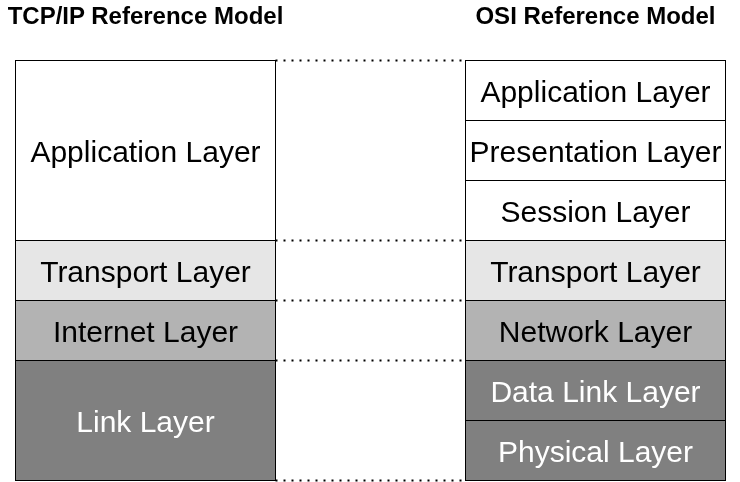
\includegraphics[width=0.5\textwidth]{assets/chap_1/osi_iso.png}
\end{figure}
\medskip

\noindent
\begin{itemize}
    \item Presentation Layer $\rightarrow$ defines format of the data so receiver can understand it (data format).
    \item Session Layer $\rightarrow$ establishes, maintains, and terminates the connection between applications (dialogue).
    \item Data Link Layer $\rightarrow$ groups raw bits into frames, handles MAC address \& check errors (local logic).
    \item Physical Layer $\rightarrow$ transmits 1s and 0s (bit) over the wire (raw signal).
\end{itemize}
\medskip

\noindent
\underline{Self-note:}
\medskip

\noindent
$\Rightarrow$ Model OSI là model hoàn chỉnh hơn so với TCP/IP.

\begin{itemize}
    \item OSI hơn 2 layer so với TCP/IP; trong đó có 2 layer được thêm vào là Session Layer và Presentation Layer, với modify lại Link Layer thành Data Link Layer và Physical Layer.
    \item Trên thực tế, người ta dùng TCP/IP nhiều hơn, do nhanh hơn (vì có ít layer và đỡ phức tạp hơn). OSI rất phức tạp nhưng đầy đủ, nên sử dụng chủ yếu trong giảng dạy.
\end{itemize}
\medskip

\subsection{OSI Model Concepts}

\noindent
\underline{Self-note:} OSI nghĩa là Open Systems Interconnection $\rightarrow$ là một khung khái niệm chia các chức năng truyền thông mạng thành 7 lớp.

$\Rightarrow$ Là mô hình quan trọng do nó chuẩn hóa cách mạng hoạt động, chia nhỏ quá trình truyền thông mạng phức tạp thành 7 tầng dễ quản lý.
\medskip

\noindent
Central concepts:

\begin{itemize}
    \item Service $\rightarrow$ define what layer does.
    \item Interfaces $\rightarrow$ defines how to access.
    \item Protocols $\rightarrow$ defines how the layer is implemented (communication).
\end{itemize}
\medskip

\subsection{Physical Layer}

\noindent
$\rightarrow$ Main concept: raw signal with 0s and 1s.

\begin{itemize}
    \item Sender $\rightarrow$ signals are modulated (điều chỉnh) onto the medium.
    \item Receiver $\rightarrow$ signals are demodulated (giải điều chỉnh) from the medium.
\end{itemize}
\medskip

\noindent
\underline{Self-note:}
\medskip

\begin{center}
\begin{tikzpicture}[>=stealth, font=\small]
    \node[align=center] (sender) at (0,0) {data\\send};
    \node[draw, minimum width=3cm, minimum height=1cm, align=center]
        (wave) at (6,0) {Sóng, tần số để truyền};
    \node[align=center] (receiver) at (12,0) {data\\received};
    \draw[->, thick, shorten >=5pt, shorten <=5pt]
        (sender.east) -- (wave.west)
        node[midway, above]{modulated};
    \draw[->, thick, shorten >=5pt, shorten <=5pt]
        (wave.east) -- (receiver.west)
        node[midway, above]{demodulated};
\end{tikzpicture}
\end{center}
\medskip

\noindent
\underline{Finalize:}
\medskip

\noindent
The core function: moving bits.

\begin{itemize}
    \item Raw transmission $\rightarrow$ to transmit the raw stream of 1s and 0s.
    \item Physical connection $\rightarrow$ defines the physical specifications for the connection (quy định các thông số kĩ thuật cho connection; ví dụ: hình dạng đầu cắm dây cáp, loại dây cáp).
\end{itemize}

\subsection{Data Link Layer}

\noindent
$\rightarrow$ Main concept: group into frames, handle transmission errors (with checksums), specifies physical network address (MAC address).
\medskip

\begin{itemize}
    \item Sender $\rightarrow$ pack the newtwork into frames and transmits them via a physical network from one device to another.
    \item Receiver $\rightarrow$ identifies frames in the bit stream from the Physical Layer.
\end{itemize}
\medskip

\noindent
\underline{Self-note:}
\medskip

\noindent
Frame (khung dữ liệu) $\rightarrow$ dùng để chứa dữ liệu và vận chuyển nó qua đường dây vật lý (physical link) hoặc sóng vô tuyến (wireless) từ sender đến receiver trong cùng một network.
\medskip

\noindent
$\rightarrow$ Tầng liên kết (data link layer) nhận một gói tin (packet) từ tầng mạng ở trên, sau đó gắn header ở trên và trailer ở dưới.
\medskip

\noindent
\underline{Finalize:}
\medskip

\noindent
The core function: Node-to-Node Delivery.

\begin{itemize}
    \item Local Delivery $\rightarrow$ to move the data between 2 devices connected to the same physical medium (ví dụ: Laptop $\rightarrow$ Switch $\rightarrow$ Router).
    \item Framing $\rightarrow$ takes the raw stream of bits from the physical layer and organizes them into distinct "sentences" called frames (gom các tín hiệu rời rạc thành các gói dữ liệu).
\end{itemize}
\medskip

\subsection{Network Layer}

\noindent
$\rightarrow$ Main concept: connects different neworks together.
\medskip

\noindent
$\rightarrow$ It doesn't care about the MAC address; only cares the IP to connect with WAN.
\medskip

\begin{itemize}
    \item Sender $\rightarrow$ packs the segments of the Transport Layer in packets.
    \item Receiver $\rightarrow$ unpacks the packets in the frames from the Data Link Layer; \textbf{routers} and \textbf{Layer-3-Switches} connect logical networks.
    \item Usually the connectionless IP is used $\rightarrow$ other protocols have been replaced by IP (e.g., IPX).
\end{itemize}

\noindent
\textbf{$\Rightarrow$ 3 main tasks:}

\begin{itemize}
    \item Logical addressing.
    \item Routing.
    \item Encapsulation.
\end{itemize}

\noindent
\underline{Finalize:}
\medskip

\noindent
The core function: Routing and Addressing.

\begin{itemize}
    \item Internetworking $\rightarrow$ to forward packets between sender and receiver in the network.
    \item Logical Addressing $\rightarrow$ uses IP addresses to identify devices $\Rightarrow$ unlike MAC addresses, IP addresses are assigned based on where you are in the network (MAC address xác định danh tính của Card mạng (NIC)). Ví dụ, IP sẽ hỏi là "máy tính mày đang ở đâu?", trong khi đó MAC sẽ hỏi là "đâu là cái máy nào của mày đang dùng dây?".
\end{itemize}
\medskip

\subsection{Transport Layer}

\noindent
$\rightarrow$ Main concept: ensures the network get the correct application.
\medskip

\begin{itemize}
    \item Sender $\rightarrow$ packs the data of the Application Layer into segments.
    \item Receiver $\rightarrow$ unpacks the segments inside the packets from the network layer.
    \item Addresses process with \textbf{port number}.
\end{itemize}
\medskip

\noindent
\textbf{$\rightarrow$ Main task:} end-to-end communication between processes.
\medskip

\noindent
$\rightarrow$ Because the computer receive thousands of packets every seconds $\Rightarrow$ it uses port to identify.
\medskip

\noindent
\textbf{2 main modes:}

\begin{itemize}
    \item Connection-oriented (TCP) $\rightarrow$ reliable, stateful $\Rightarrow$ ensure data arrives prefectly.
    \item Connectionless (UDP) $\rightarrow$ unreliable, stateless, fast $\Rightarrow$ no guarantee of delivery.
\end{itemize}
\medskip

\noindent
\underline{Self-note:}

\begin{itemize}
    \item TCP $\rightarrow$ nó đảm bảo đủ data qua $\Rightarrow$ tốn thời gian (ví dụ: download file nào đó).
    \item UDP $\rightarrow$ nó đảm bảo kịp tiến độ truyền qua $\Rightarrow$ dễ thiếu data (ví dụ: voice call).
\end{itemize}

\noindent
\underline{Finalize:}
\medskip

\noindent
The core function: End-to-End Communication.

\begin{itemize}
    \item Process-to-Process $\rightarrow$ to transport segments between specific processes (applications) on different devices.
    \item Port numbers $\rightarrow$ uses to identify which application should receive the data (phân chia gói tin vào các ứng dụng).
\end{itemize}
\medskip

\subsection{Session Layer}

\noindent
$\rightarrow$ Main concept: dialogue control: setup, manage, and terminate connections (sessions).
\medskip

\noindent
\underline{The Problem:} Nếu dung lượng 5GB nhưng mà nó download tới 4.9GB thì rớt mạng. Phải làm sao?

$\Rightarrow$ Không có session layer thì nó sẽ download lại từ con số 0 (cho nó không có checkpoint).
\medskip

\noindent
\textbf{$\rightarrow$ 3 main tasks:}

\begin{itemize}
    \item Checkpointing (and recovery).
    \item Authentication.
    \item Authorization.
\end{itemize}

\noindent
\underline{Self-note:} Trong TCP/IP, người ta cho cái layer này vào trực tiếp cái Application Layer, ví dụ như dùng cookie để maintain session.
\medskip

\noindent
\underline{Finalize:}
\medskip

\noindent
The core function: dialogue control $\rightarrow$ to setup, maintain, and terminate connections (sessions) between applications.

\begin{itemize}
    \item Synchronization $\rightarrow$ decides whose turn it is to speak and keep the data stream organized (thiết lập \& quản lý các phiên làm việc giữa các ứng dụng).
    \item State Management $\rightarrow$ tracks if the connection is active, idle, or broken.
    \item security $\rightarrow$ xác thực và cấp quyền trước khi bắt đầu một connection.
\end{itemize}

\subsection{Presentation Layer}

\noindent
$\rightarrow$ Defines format (presentation) of the data.
\medskip

\noindent
\underline{The Problem:} một bên dùng ASCII để render text, còn một bên dùng EBCDIC. Phải làm sao?

$\Rightarrow$ Phải có layer này để cho ra common format (format chung) mới có thể giao tiếp được.
\medskip

\noindent
\textbf{$\rightarrow$ 3 main tasks:}

\begin{itemize}
    \item Translation $\rightarrow$ connect to standard format.
    \item Encryption $\rightarrow$ security.
    \item Compression $\rightarrow$ smaller data for faster travelling.
\end{itemize}

\noindent
\underline{Finalize:}
\medskip

\noindent
The core function: Formatting and Syntax $\rightarrow$ to define the format (presentation) of the data.

\begin{itemize}
    \item Translation $\rightarrow$ đảm bảo máy tính nhận hiểu được dữ liệu mà máy tính gửi truyền đi.
    \item Encryption $\rightarrow$ đảm nhận việc mã hóa dữ liệu để tăng tính bảo mật.
    \item Compression $\rightarrow$ thu gọn dữ liệu để truyền nhanh hơn.
\end{itemize}

\subsection{Application Layer}

\noindent
$\rightarrow$ User interaction.
\medskip

\noindent
\textbf{$\rightarrow$ 2 main tasks:}

\begin{itemize}
    \item The payload $\rightarrow$ holds actual data we care.
    \item Semantics $\rightarrow$ focus on the meaning and logic of the application (don't care about IP addressses, cables, or routing).
\end{itemize}

\noindent
\underline{Self-note:}
\medskip

\noindent
DNS nghĩa là Domain Name Server.
\medskip

\begin{figure}[h]
    \centering
    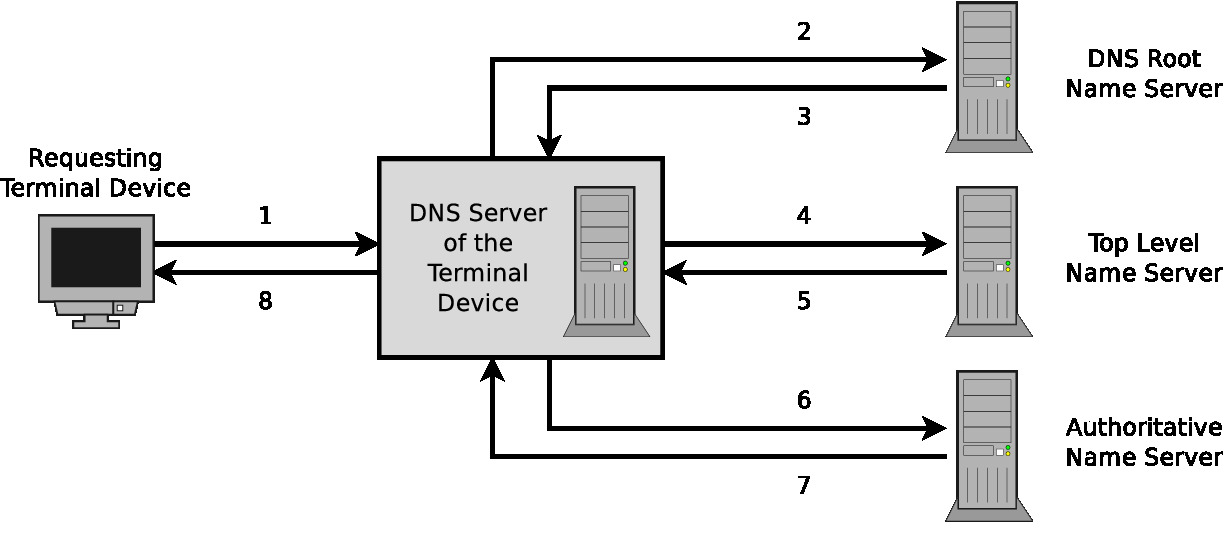
\includegraphics[width=0.55\textwidth]{assets/chap_1/dns_illust.jpg}
\end{figure}
\medskip

\noindent
$\rightarrow$ Tóm tắt DNS: Client $\rightarrow$ Root $\rightarrow$ TLD $\rightarrow$ Authoritative $\rightarrow$ nhận IP.
\medskip

\begin{center}
\begin{tikzpicture}[
    box/.style={draw, minimum width=3.5cm, minimum height=1cm, align=center},
    >=stealth
]
\node[box] (root) at (0,0) {\textbf{Root Name Server} \\ (máy chủ tên miền gốc)};
\node[box] (tld)  at (0,-2) {\textbf{TLD Server (.com/.net/.vn)} \\ (Top-Level Domain Server; \\ máy chủ tên miền cấp cao)};
\node[box] (auth) at (0,-4) {\textbf{Authoritative Name Server} \\ (máy chủ tên miền thẩm quyền)};
\draw[->, thick] (-3,0) node[left, align=center]{Client Query \\ (truy vấn từ \\ máy khách)} -- (root.west)
    node[midway, above]{1};
\draw[->, thick] (root) -- (tld)
    node[midway, right]{2};
\draw[->, thick] (tld) -- (auth)
    node[midway, right]{3};
\draw[<-, thick] (root.east) -- (3,0) node[right, align=left]{Root referral \\ (chuyển hướng từ \\ máy chủ gốc)};
\draw[<-, thick] (tld.east) -- (3,-2) node[right, align=left]{TLD referral \\ (chuyển hướng từ \\ máy chủ TLD)};
\draw[<-, thick] (auth.east) -- (3,-4) node[right, align=left]{Final answer \\ (nhận IP)};
\end{tikzpicture}
\end{center}
\medskip

\noindent
\underline{The Problem:} Computers communicate using numbers called IP address, but we can't remember them. What can we do?

$\Rightarrow$ We prefer like \texttt{google.com}, etc.
\medskip

\noindent
$\Rightarrow$ DNS translates (resolves) the human-readable Domain Names into machine readable IP address.
\medskip

\noindent
\underline{Finalize:}
\medskip

\noindent
The core function: user interaction $\rightarrow$ contains all protocols that interact directly with application programs.

\begin{itemize}
    \item The payload (giao diện người dùng) $\rightarrow$ chứa các giao thức để communicate giữa phần mềm trong network.
    \item Semantics (ngữ nghĩa) $\rightarrow$ chứa nội dung muốn gửi (content).
\end{itemize}
\medskip

\section{Topologies}

\subsection{Topologies of Computer Networks}

\noindent
$\rightarrow$ Mô tả cách bố trí \& kết nối các thiết bị trong network.
\medskip

\noindent
Large-scale network is often a combination of different topologies. Physical and Logical topology may differ:

\begin{itemize}
    \item Physical topology $\rightarrow$ actual layout of the devices (cách đi dây thực tế).
    \item Logical topology $\rightarrow$ how data flows within the network (cách data di chuyển trong network).
\end{itemize}
\medskip

\noindent
Topologies are graphically represented with nodes and edges.
\medskip

\subsection{Bus Network}

\begin{figure}[h]
    \centering
    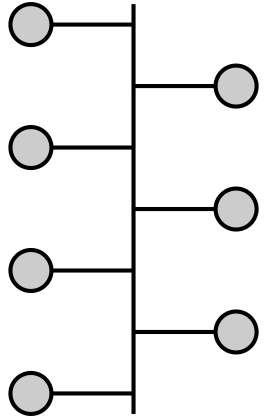
\includegraphics[width=0.13\textwidth]{assets/chap_1/bus_net.png}
\end{figure}
\medskip

\noindent
$\rightarrow$ Tất cả các thiết bị được kết nối vào một đường dây truyền dẫn chung gọi là Bus $\Rightarrow$ không có thiết bị trung tâm nào ở giữa.
\medskip

\begin{itemize}
    \item \textbf{Pros:} cheap.
    \item \textbf{Cons:} dây cáp chính đứt $\rightarrow$ dead; một thời điểm chỉ có 1 máy gửi dữ liệu, 2 máy gửi cùng lúc sẽ bị collision.
\end{itemize}
\medskip

\subsection{Ring Network}

\begin{figure}[h]
    \centering
    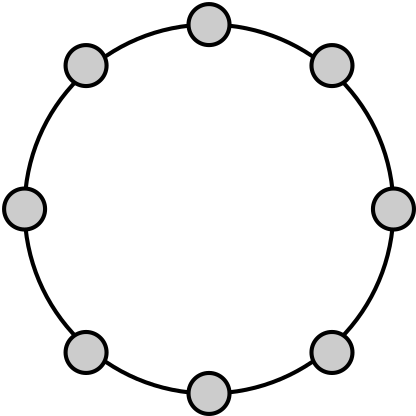
\includegraphics[width=0.2\textwidth]{assets/chap_1/ring_net.png}
\end{figure}
\medskip

\noindent
$\rightarrow$ Mỗi nút nối với đúng 2 nút khác, tạo thành một vòng khép kín, dữ liệu truyền 1 chiều từ nút này sang nút khác.
\medskip

\begin{itemize}
    \item \textbf{Pros:} mỗi nút hoạt động như một bộ khuếch đại (repeater) $\rightarrow$ tín hiệu có thể truyền đi xa hơn.
    \item \textbf{Cons:} một dây đứt or 1 máy hỏng $\rightarrow$ dead (trừ khi dùng vòng kép dự phòng).
\end{itemize}
\medskip

\subsection{Star Network}

\begin{figure}[h]
    \centering
    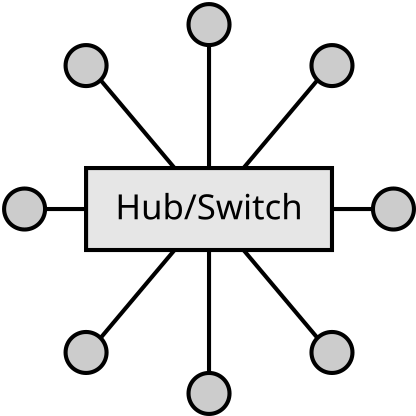
\includegraphics[width=0.2\textwidth]{assets/chap_1/star_net.png}
\end{figure}
\medskip

\noindent
$\rightarrow$ Tất cả các nút kết nối trực tiếp vào 1 thiết bị trung tâm (Hub / Switch).
\medskip

\begin{itemize}
    \item \textbf{Pros:} stable $\rightarrow$ 1 máy or dây bị hư vẫn hoạt động bình thường; dễ mở rộng $\rightarrow$ thêm dây vào Switch là có thể thêm máy để hoạt động.
    \item \textbf{Cons:} nếu Switch hỏng $\rightarrow$ dead.
\end{itemize}
\medskip

\subsection{Mesh Network}

\begin{figure}[h]
    \centering
    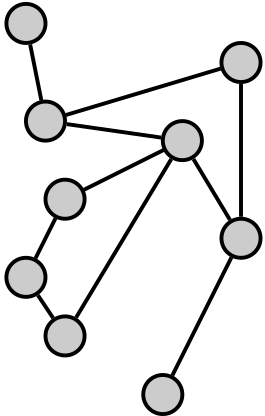
\includegraphics[width=0.15\textwidth]{assets/chap_1/mesh_net.png}
\end{figure}
\medskip

\noindent
\underline{Self-note:} mesh network nghĩa là mạng lưới.
\medskip

\noindent
$\rightarrow$ Mỗi nút được kết nối với nhiều nút khác. $\Rightarrow$ Full mesh $\rightarrow$ mọi nút được kết nối với nhau.
\medskip

\begin{itemize}
    \item \textbf{Pros:} safe $\rightarrow$ nếu bị đứt dây thì còn đường dự phòng.
    \item \textbf{Cons:} chi phí cao; đi dây phức tạp.
\end{itemize}

\subsection{Tree Network}

\begin{figure}[h]
    \centering
    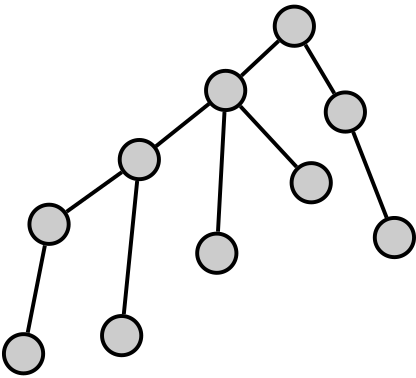
\includegraphics[width=0.2\textwidth]{assets/chap_1/tree_net.png}
\end{figure}
\medskip

\noindent
$\rightarrow$ Sự kết hợp phân cấp của star network; có nút root trên cùng.
\medskip

\begin{itemize}
    \item \textbf{Pros:} tốt cho việc quản lý các mạng lớn.
    \item \textbf{Cons:} root hỏng $\rightarrow$ các nhánh dead; dễ bị nghẽn $\rightarrow$ nếu large tree $\Rightarrow$ communication from one half of the tree to the other half must go through the root.
\end{itemize}

\pagebreak

\subsection{Cellular Network}

\begin{figure}[h]
    \centering
    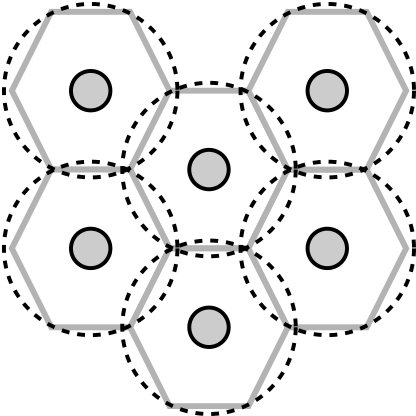
\includegraphics[width=0.22\textwidth]{assets/chap_1/cell_net.png}
\end{figure}
\medskip

\noindent
$\rightarrow$ Dùng cho mạng không dây. Mạng được chia thành các khu vực gọi là cell, mỗi cell có một trạm phủ sóng.
\medskip

\begin{itemize}
    \item \textbf{Pros:} người dùng không cần dây dẫn; node failure không bị ảnh hưởng.
    \item \textbf{Cons:} cần cơ chế tránh xung đột (collision) (CSMA/CA) do nhiều thiết bị dùng chung một tần số; bị giới hạn vùng phủ sóng (based on stations and their positions).
\end{itemize}
\medskip

\subsection{Current Situation}

\begin{itemize}
    \item LAN $\rightarrow$ dùng star network.
    \item Wireless $\rightarrow$ dùng cellular network.
    \item Lõi Internet (backbone) $\rightarrow$ dùng mesh network.
    \item Bus \& Ring $\rightarrow$ hiếm khi dùng nữa (no longer used).
\end{itemize}

\pagebreak
